\documentclass{beamer}
\usepackage[sloppy=false]{thaispec}
\usepackage{graphicx}
\usetheme{Madrid}
\graphicspath{{project_image}}
\title{แบบจำลองทางคณิตศาสตร์การเรียนรู้ตัวอักษรคันจิ}
\author{นายณัฐวุฒิ เทศงามถ้วน 116410901009-3 \\ นายคณัสนันท์ ทรัพย์อุดม 116410901033-3 \\ นายธนาคาร ธิคุณ 116410901048-1}
\date{5 เมษายน 2566}

\begin{document}
\begin{frame}
\maketitle 
\end{frame}
\begin{frame}{ที่มาเเละความสำคัญของโปรเจค}
\begin{center}
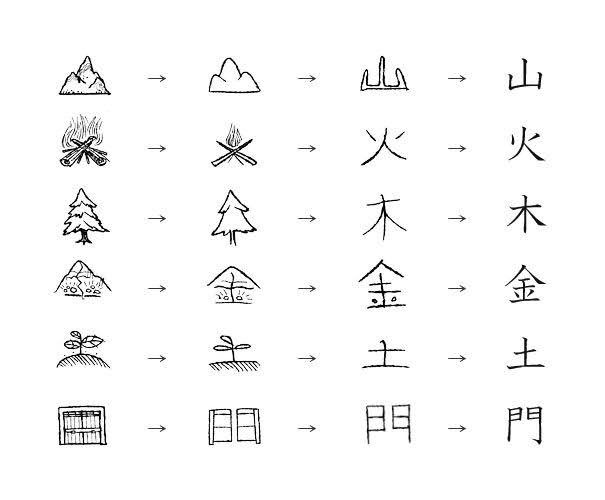
\includegraphics[scale = 0.3]{1.jpg}
\end{center}
คันจิ หมายถึง ตัวอักษรคันจิ คือ ตัวอักษรภาพที่ใช้ในการสื่อสารของประเทศจีน ญี่ปุ่น โดยเน้นการนำเสนอความหมายของคำแทนวิธีการออกเสียงของคำ
\end{frame}

\begin{frame}{ข้อมูลที่ใช้ทำโปรเจค} 
\textbf{หลักสูตรสาขาวิชาญี่ปุ่นโดยได้มาจากมหาวิทยาลัยธรรมศาสตร์มีข้อมูลดังต่อไปนี้         }
\begin{enumerate}
	\item วิชา Japanese 1 : ตัวอักษรคันจิทั้งหมด 80 ตัว 
	\item วิชา Japanese 2 : ตัวอักษรคันจิทั้งหมด 120 ตัว
	\item วิชา Japanese 3 : ตัวอักษรคันจิทั้งหมด 250 ตัว	 
	\item วิชา Japanese 4 : ตัวอักษรคันจิทั้งหมด 250 ตัว 
	\item วิชา Japanese 5 : ตัวอักษรคันจิทั้งหมด 300 ตัว  
	\item วิชา Japanese 6 : ตัวอักษรคันจิทั้งหมด 350 ตัว  
	\item คันจิที่ไม่ได้อยู่ในรายวิชา Japanese 1 ถึง Japanese 6 ให้ผู้เรียนศึกษาด้วยตนเองเป็นตัวอักษรคันจิอีก 786 ตัว
\end{enumerate}
\end{frame}

\begin{frame}{ข้อมูลที่ใช้ทำโปรเจค}
\textbf{The Forgetting Curve }
\begin{center}
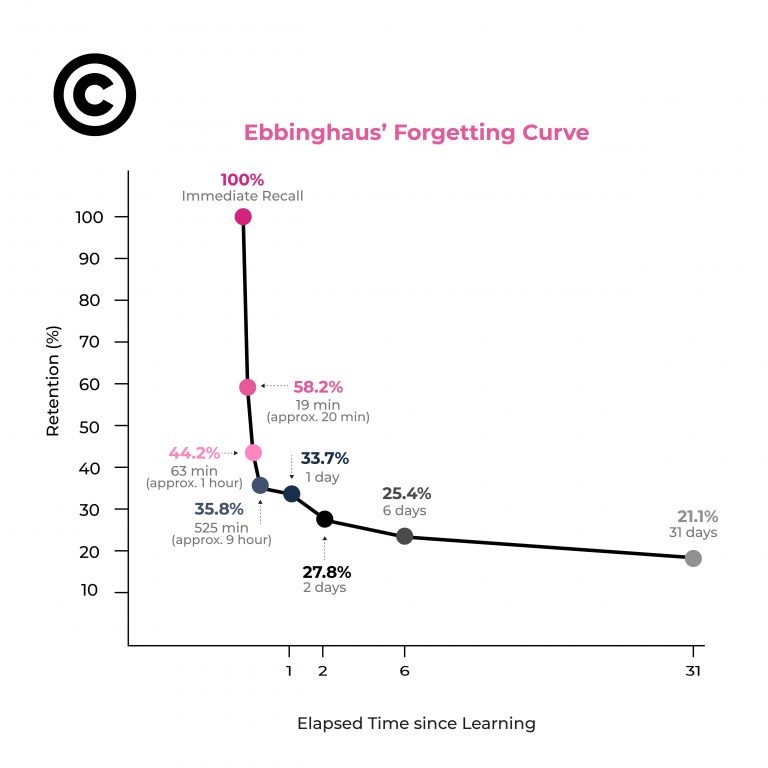
\includegraphics[scale = 0.4]{2.jpg}
\end{center}
\end{frame}

\begin{frame}{ผลลัพธ์หลัก : ปัญหา }
การหาสมการที่ใช้ทำนายผลการเรียนรู้ตัวอักษรคันจิและถ้าต้องการเรียนรู้ตัวอักษรคันจิภายในระยะเวลา 720 วัน จะต้องเรียนรู้ตัวอักษรคันจิกี่ตัวต่อวันถึงจะเรียนรู้ตัวอักษรคันจิครบทั้งหมด 2136 ตัว
\end{frame}

\begin{frame}{แบบจำลองทางคณิตศาสตร์ : องค์ประกอบ}

\begin{table}
\centering
\scalebox{0.7}{
\begin{tabular}{ |c|c|c|c| }
\hline
\textbf{สัญลักษณ์ } & \textbf{ประเภท } & \textbf{ตัวแปร } & \textbf{หน่วย } \\
\hline
$L(t)$ & ตัวแปรผลลัพธ์ & ตัวอักษรคันจิที่ผู้ศึกษารู้ ณ วันที่ t & ตัว \\
\hline
$L_i(t)$ & พารามิเตอร์ & ตัวอักษรคันจิที่ผู้ศึกษารู้ในช่วงเวลาเรียน Japanese i ณ วันที่ t & ตัว \\
\hline
$K_i$ & พารามิเตอร์ & ตัวอักษรคันจิที่สามารถเรียนรู้ได้ด้วยตนเอง ณ เวลาเรียน Japanese i & ตัว \\
\hline
$t$ & ตัวแปรนำเข้า & เวลาในการเรียนรู้ตัวอักษรคันจิ & วัน \\
\hline 
$J_i$ & พารามิเตอร์ & ตัวอักษรคันจิทั้งหมดที่สามารถเรียนรู้ได้ในช่วงเวลาเรียน Japanese i & ตัว \\
\hline
$K_{0,i}$ & พารามิเตอร์ & ตัวอักษรคันจิที่ผู้ศึกษามีความรู้และจำได้อยู่แล้วในวิชา Japanese i & ตัว \\
\hline
$\alpha$ & พารามิเตอร์ & ความสามารถในการเรียนรู้ตัวอักษรคันจิต่อวัน & ตัว/วัน \\
\hline 
$\beta $ & พารามิเตอร์ & อัตราการสูญเสียตัวอักษรคันจิ & ไม่มี \\
\hline 
\end{tabular}}
\end{table}
\end{frame}

\begin{frame}{แบบจำลองทางคณิตศาสตร์ : สมมุติฐาน} 
\begin{enumerate}
	{\scriptsize
	\item เวลาที่ใช้ในการเรียนรู้ตัวอักษรคันจิจะใช้เวลาเรียนทั้งหมด 6 ภาคเรียน ภาคเรียนละ 4 เดือน และเดือนละ 30 วัน โดยกำหนดให้การเรียน Japanese 1 อยู่ในช่วงเวลาวันที่ 1 ถึงวันที่ 120 Japanese 2 อยู่ในช่วงเวลาวันที่ 121 ถึงวันที่ 240 Japanese 3 อยู่ในช่วงเวลาวันที่ 241 ถึงวันที่ 360 Japanese 4 อยู่ในช่วงเวลาวันที่ 361 ถึงวันที่ 480 Japanese 5 อยู่ในช่วงเวลาวันที่ 481 ถึงวันที่ 600 Japanese 6 อยู่ในช่วงเวลาวันที่ 601 ถึงวันที่ 720 และตัวอักษรคันจิที่ไม่ได้อยู่ในรายวิชาสามารถเรียนได้ภายในช่วงเวลา 6 ภาคเรียน
	\item การเรียนรู้ตัวอักษรคันจิในแต่ละวันสามารถหลงลืมตัวอักษรคันจิที่เคยเรียนรู้ได้ด้วยหลักการ The Forgetting Curve
	\item ผู้เรียนคันจิอยู่ในสถานะที่เรียนรู้ตัวอักษรคันจิตลอดเวลา เนื่องจากสภาวะการเรียนรู้ภาษาญี่ปุ่นต้องใช้เวลาไปกับการอยู่กับตัวอักษรคันจิเป็นจำนวนมากเพื่อให้คุ้นเคยกับภาษาญี่ปุ่นตลอดเวลา
	\item เวลาที่ใช้ในการเรียนรู้ตัวอักษรคันจิจะไม่นับเวลาช่วงปิดเทอมเข้ามาเกี่ยวข้อง โดยถือว่าการเรียนรู้ตัวอักษรคันจิจะเรียนรู้แบบต่อเนื่องจนกว่าจะครบทั้งหมด 6 ภาคเรียน}
\end{enumerate}

\end{frame}


\begin{frame}{แบบจำลองทางคณิตศาสตร์} 
กำหนดให้ $ K_i , K_{0,i} , t \in \mathbb{N}_+ , \alpha , \beta \in \mathbb{R}_+ $ และ 
$$ L(t) = L_1(t) + L_2(t) + L_3(t) + L_4(t) + L_5(t) + L_6(t) $$
โดยที่ 
\begin{center}
\begin{align*}
L_1(t) & = \min \{J_1 + K_1, \left\lfloor (1 - \beta)(K_{0,1} + \alpha{t}) \right\rfloor\} \; ; t \in [0,120] \\
L_2(t) & = \min \{J_2 + K_2, \left\lfloor (1 - \beta)(K_{0,2} + \alpha{(t - 120)}) \right\rfloor\} \; ; t \in (120,240] \\
L_3(t) & = \min \{J_3 + K_3, \left\lfloor (1 - \beta)(K_{0,3} + \alpha{(t - 240)}) \right\rfloor\} \; ; t \in (240,360] \\
L_4(t) & = \min \{J_4 + K_4, \left\lfloor (1 - \beta)(K_{0,4} + \alpha{(t - 360)}) \right\rfloor\} \; ; t \in (360,480] \\
L_5(t) & = \min \{J_5 + K_5, \left\lfloor (1 - \beta)(K_{0,5} + \alpha{(t - 480)}) \right\rfloor\} \; ; t \in (480,600] \\
L_6(t) & = \min \{J_6 + K_6, \left\lfloor (1 - \beta)(K_{0,6} + \alpha{(t - 600)}) \right\rfloor\} \; ; t \in (600,720]
\end{align*}
\end{center}
\end{frame}

\begin{frame}{แบบจำลองทางคณิตศาสตร์ : หา $\alpha$ ที่เหมาะสม }
กำหนดให้ $ K_i , K_{0,i} \in \mathbb{N}_+ , \alpha , \beta \in \mathbb{R}_+ $ และ $t = 720$
{\tiny 
\begin{align*}
2136 & = \left\lfloor(1 - \beta)(\sum_{i=1}^{6} K_{0,i} + \alpha{t})\right\rfloor\ \\
2136 & = \left\lfloor(1 - \beta)(\sum_{i=1}^{6} K_{0,i} + 720\alpha)\right\rfloor\ \\
2136 & \leq (1 - \beta)(\sum_{i=1}^{6} K_{0,i} + 720\alpha < 2137 \\
\frac{2136}{(1 - \beta)} & \leq \sum_{i=1}^{6} K_{0,i} + 720\alpha < \frac{2137}{(1 - \beta)} \\
\frac{2136}{(1 - \beta)} - \sum_{i=1}^{6} K_{0,i} & \leq 720\alpha < \frac{2137}{(1 - \beta)} - \sum_{i=1}^{6} K_{0,i} \\
\frac{2136}{720(1 - \beta)} - \frac{\sum_{i=1}^{6} K_{0,i}}{720} & \leq \alpha < \frac{2137}{720(1 - \beta)} - \frac{\sum_{i=1}^{6} K_{0,i}}{720} \\ 
\frac{2136 - (\sum_{i=1}^{6} K_{0,i})(1 - \beta)}{720(1 - \beta)} & \leq \alpha < \frac{2137 - (\sum_{i=1}^{6} K_{0,i})(1 - \beta)}{720(1 - \beta)}
\end{align*}
}%
\end{frame}

\begin{frame}{ผลลัพธ์เชิงตัวเลขแบบทั่วไป} 
\begin{center}
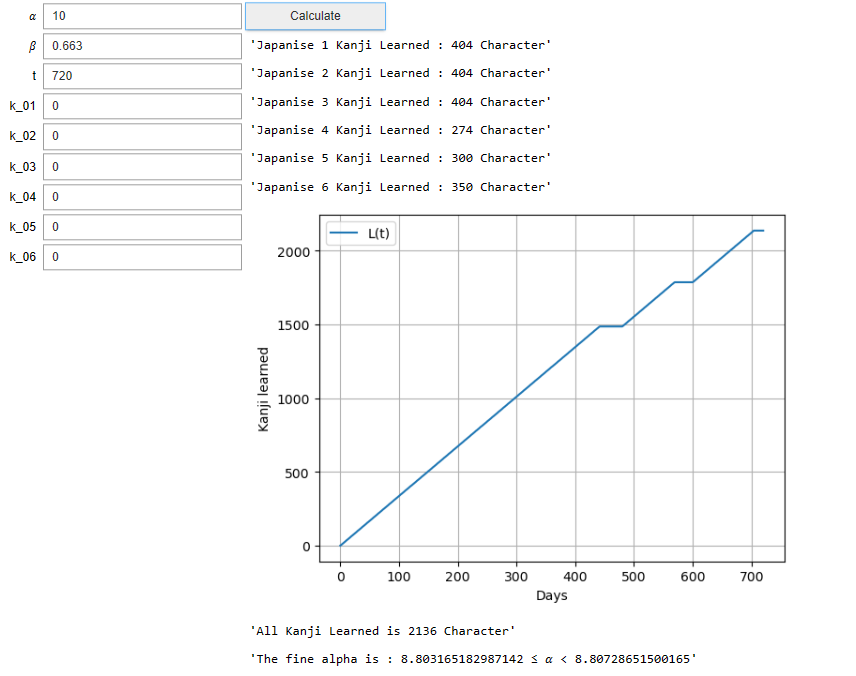
\includegraphics[scale = 0.3]{3.png}
\end{center}
\end{frame}

\begin{frame}{ผลลัพธ์เชิงตัวเลขแบบพอดี} 
\begin{center}
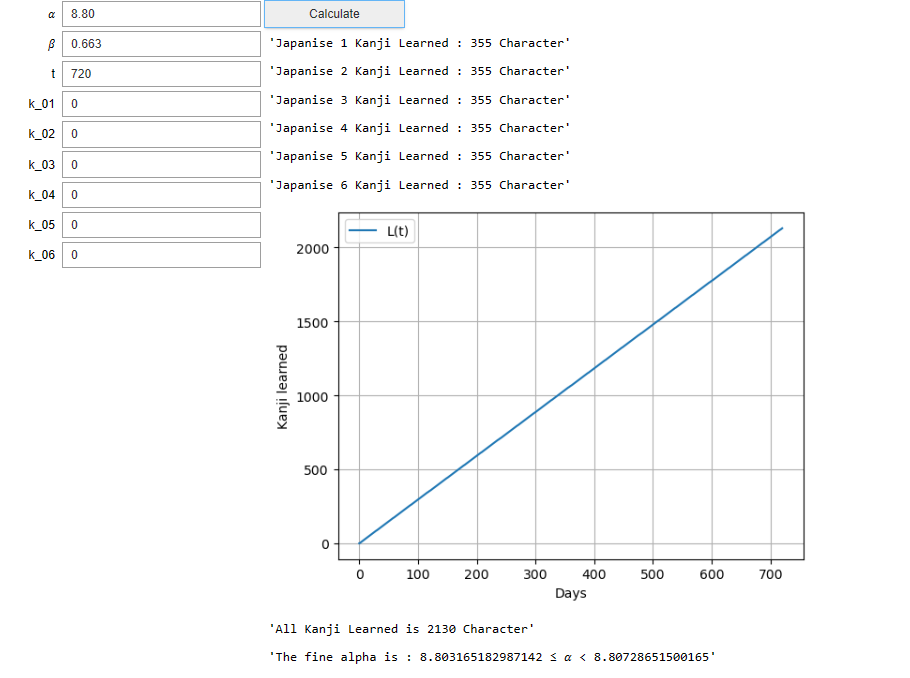
\includegraphics[scale = 0.3]{4.png}
\end{center}
\end{frame}

\begin{frame}{ผลลัพธ์เชิงตัวเลขแบบไม่พอดี} 
\begin{center}
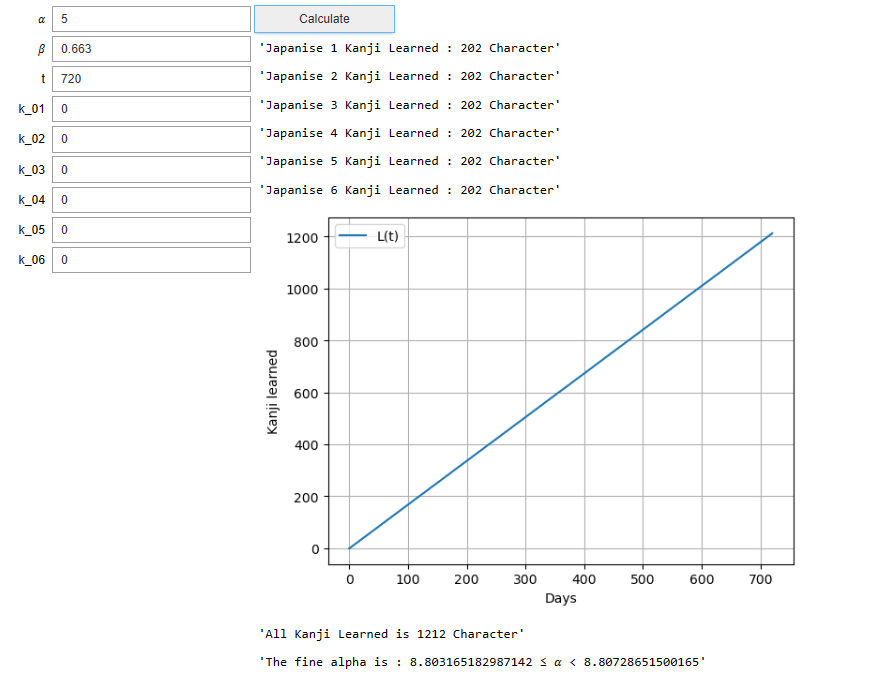
\includegraphics[scale = 0.3]{5.png}
\end{center}
\end{frame}

\begin{frame}{ผลลัพธ์เชิงตัวเลขแบบพิเศษ} 
\begin{center}
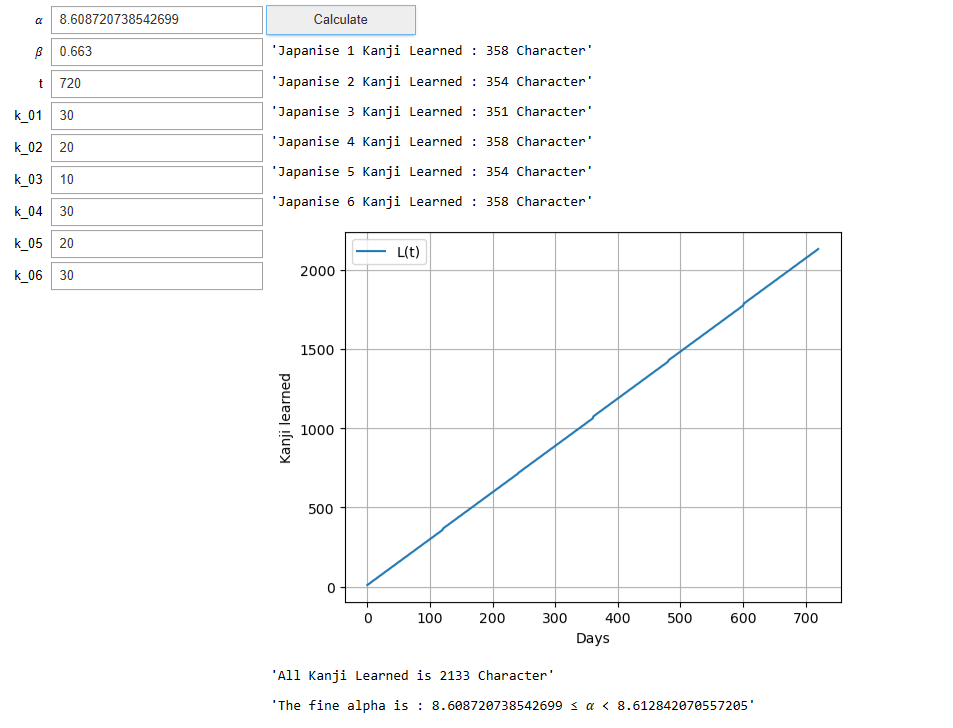
\includegraphics[scale = 0.3]{6.png}
\end{center}
\end{frame}

\begin{frame} {สรุป}
จากการทำแบบจำลองทางคณิตศาสตร์การเรียนรู้ตัวอักษรคันจิ ทำให้เราพบว่าแบบจำลองทางคณิตศาสตร์ของเราสามารถบรรลุ โจทย์การหาเวลาในการเรียนรู้ตัวอักษรคันจิเท่าไร จึงจะเรียนรู้ครบทุกตัวอักษรคันจิและการหาจำนวนตัวอักษรคันจิที่ควรเรียน ต่อวันเมื่อมีเวลาในการเรียนที่จำกัด
\end{frame}

\end{document}